\begin{figure}[H]
\centering
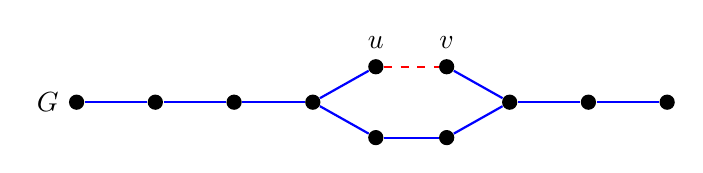
\begin{tikzpicture}[
  dot/.style={circle, fill=black, inner sep=0pt, minimum size=5.5pt},
  blue edge/.style={blue, thick},
  red dashed/.style={red, thick, dashed}
]

  % Left linear path
  \node[dot, label=left:$G$] (g) at (0,0) {};
  \node[dot] (n2) at (1,0) {};
  \node[dot] (n3) at (2,0) {};
  \node[dot] (split) at (3,0) {};

  % Cycle nodes
  \node[dot, label=above:$u$] (u) at (3.8, 0.45) {};
  \node[dot, label=above:$v$] (v) at (4.7, 0.45) {};
  \node[dot] (b1) at (3.8, -0.45) {};
  \node[dot] (b2) at (4.7, -0.45) {};

  % Right linear path
  \node[dot] (merge) at (5.5, 0) {};
  \node[dot] (n10) at (6.5, 0) {};
  \node[dot] (n11) at (7.5, 0) {};

  % Blue solid edges
  \draw[blue edge] (g) -- (n2) -- (n3) -- (split);
  \draw[blue edge] (split) -- (u);
  \draw[blue edge] (split) -- (b1);
  \draw[blue edge] (b1) -- (b2);
  \draw[blue edge] (v) -- (merge);
  \draw[blue edge] (b2) -- (merge);
  \draw[blue edge] (merge) -- (n10) -- (n11);

  % Red dashed edge
  \draw[red dashed] (u) -- (v);

\end{tikzpicture}
\end{figure}
